\section{Results}\label{sec:results}


\subsection{Base variance predictions}

Figure \ref{fig:histogram} shows a histogram with the variance distribution on correct and incorrect predictions. From this histogram, one can observe that the model's classification is almost always correct when it is paired with a low variance prediction. The higher the model's predicted variance becomes, the more often the classification is incorrect. Although the two histograms overlap, there is a clear skew towards higher variances for the incorrect predictions. On the highest variance predictions ranging from $0.24$ to $0.25$, the distribution between correct and incorrect classifications is nearly equal, indicating that the model is randomly guessing the classification.

\begin{figure}[!tbp]
    \centering
        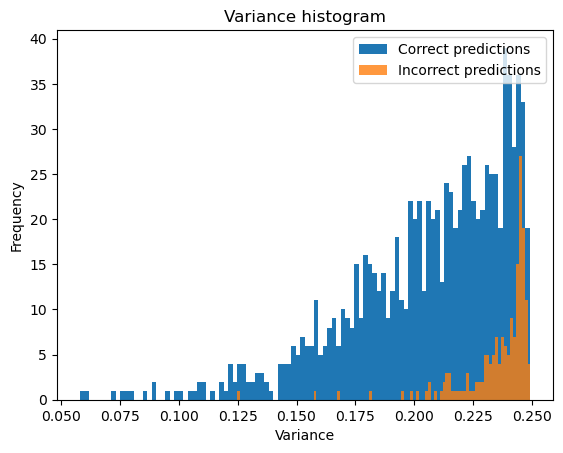
\includegraphics[width=7.7cm]{img/histogram.png}
    \caption{Histogram with the frequencies of variance predictions for correct and incorrect predictions.}
    \label{fig:histogram}
\end{figure}


\subsection{General noise}

Figure \ref{fig:label_shuffle} shows the effect of shuffling the labels of training and testing data on the model's predicted variance. Here, it is clear that there is an increase in variance as more labels in the training and testing set are shuffled. However, this difference is not very large, as there is only an increase of approximately $0.027$, with relatively high variance between runs. However, the overall increasing behavior of the variance's head output is as expected. It indicates that the model is working as intended and is predicting the variance based on the quality of the input.

\begin{figure}[!tbp]
    \centering
        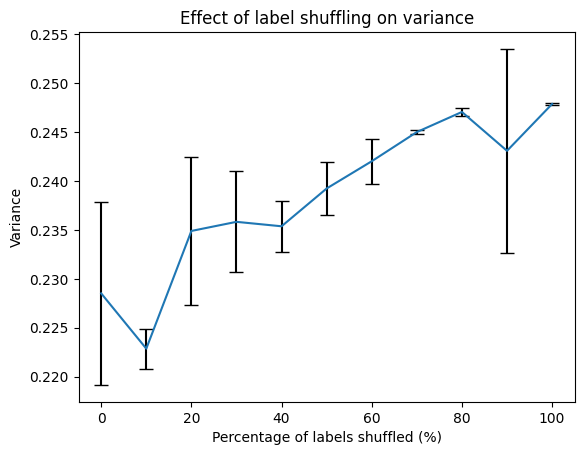
\includegraphics[width=7.7cm]{img/label_shuffle.png}
    \caption{The effect of label shuffling on the output of the variance head.}
    \label{fig:label_shuffle}
\end{figure}


Figure \ref{fig:general} shows two measurements of the model. The two leftmost plots show the predicted variance of the model, whereas the two rightmost plots show the model's accuracy. The top plots show the behavior when Gaussian noise is added to the entire length of the signal, whereas the bottom plots show the behavior when channels are entirely zeroed. The x-axis here represents the \verb|severity|, which indicates the strength of the noise. Higher values indicate that the added noise is of higher magnitude (in the case of Gaussian noise), occurring in more channels per episode and affecting more episodes in general.

As can be seen from these plots, there is a clear increase in the predicted variance as the severity of the noise increases. This increase is present for the Gaussian noise and zeroing methods. Secondly, there is a clear decrease in accuracy as the severity of the noise increases. This behavior is also present for both types of noise. However, like the previous experiment, it is paired with a high variance between runs.

\begin{figure}[!tbp]
    \centering
        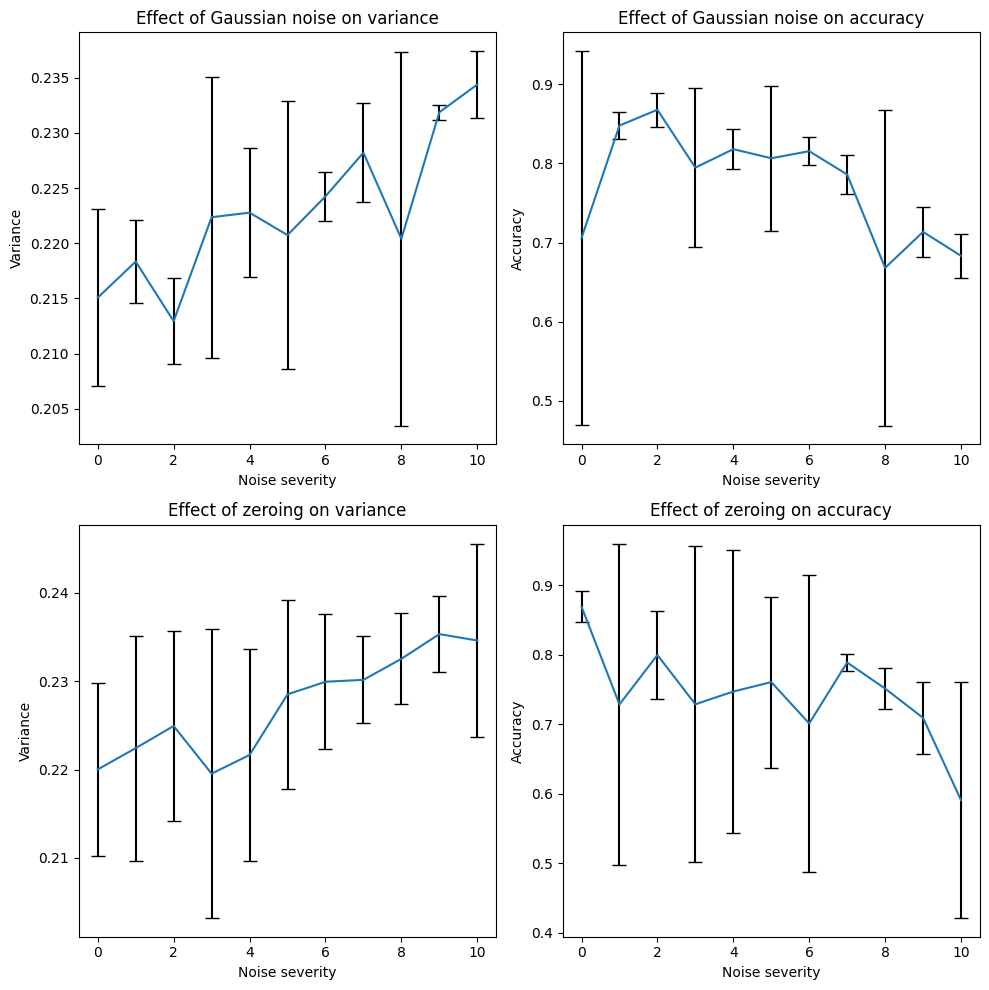
\includegraphics[width=7.7cm]{img/general.png}
    \caption{The effect of different intensities of artificial noise added to the entire signal length on the model's accuracy and variance.}
    \label{fig:general}
\end{figure}

\subsection{Localized noise}

Figure \ref{fig:local} shows the influence of the location to which the noise has been added on both the variance and accuracy of the model. The leftmost plots show the predicted variance of the model, whereas the rightmost plots show the model's accuracy. The top plots show the behavior when Gaussian noise is added to the data, whereas the bottom plots show the behavior when channels are zeroed. The leftmost column shows the effect of the noise being added on the 0-250ms region, whereas the rightmost column shows the effect of the noise being added on the 250-500ms region.

As can be observed from these plots, the general trend for both models is that the variance is higher when noise is added to the 250-500 ms region than the 0-250 ms region. The accuracy is slightly lower when the noise is added to the 250-500 ms region than the 0-250 ms region. It also observed that zeroing has a stronger effect on the variance and accuracy than Gaussian noise. This behavior is according to expectation since a Gaussian noise corrupted signal still resembles the original signal to some extent, regardless of the degree of Gaussian noise. Moreover, when averaging many signals corrupted with Gaussian noise, the noise will balance each other out. In contrast, the zeroing of signals does not resemble the original signal. The observation that noise on the 250-500 ms region substantially influences the accuracy and variance compared to the 0-250 ms region is as expected, as previous research showed that the most prominent part of the \verb|ErrP| signal occurs within this window. 

However, the differences between these two regions in accuracy and variance are minimal and are similar to the previous experiments, paired with high variance between runs.

\begin{figure}[!tbp]
    \centering
        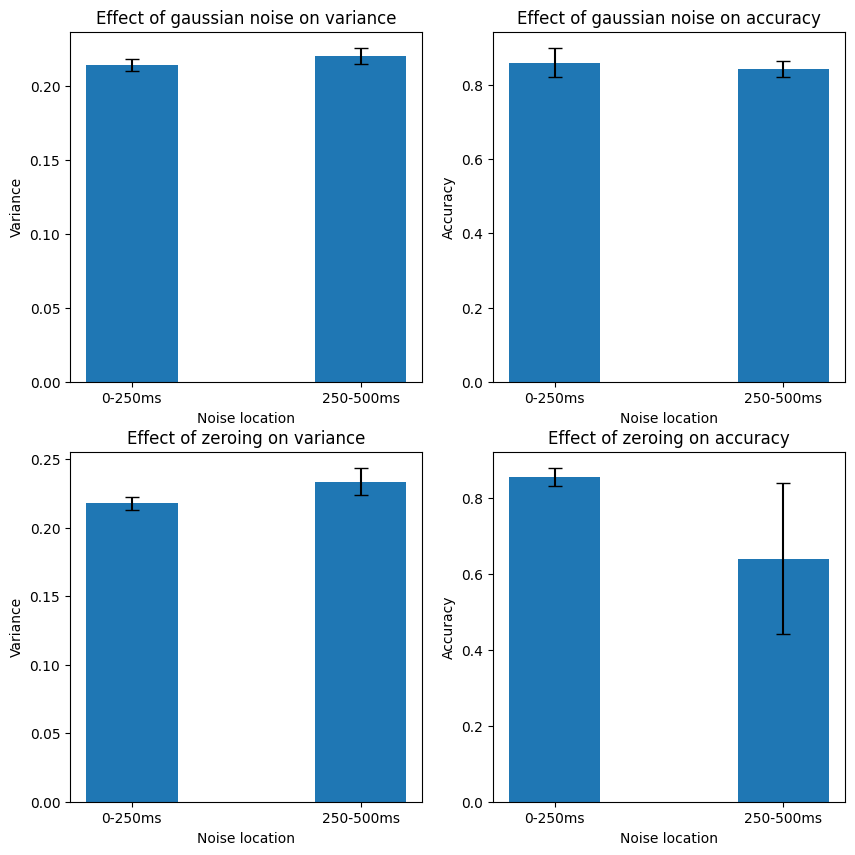
\includegraphics[width=7.7cm]{img/local.png}
    \caption{The effect of strong noise added to two different regions of the signal on the accuracy and variance of the model. The two regions tested are the ranges of 0ms to 250ms and 250ms to 500ms.}
    \label{fig:local}
\end{figure}

\subsection{Tracable noise}

Figure \ref{fig:shap} shows the single-dimensional heatmaps of the Shapley values of the predictions of the variance head. Here, the Shapley values are depicted as a continuous color palate referring to the contribution of the data points. Lighter colors (yellow) indicate a strong positive contribution to the prediction, and darker colors (blue) indicate a strong negative contribution to the variance prediction. Here, the Shapley values are averaged over all channels.

Comparing these single-dimensional heatmaps yields various observations. Firstly, there is a noticeable difference between the Shapley values of the original signals and the signals with artificial noise added to them. In the case of the Gaussian Noise variant, it is clear to which area the noise has been added due to the oscillating behavior of the Shapley values. This oscillating behavior originates from the Gaussian noise adding large differences between adjacent data points. This oscillating behavior will most likely disappear when computing and averaging the Shapley values over more episodes since the noisy signal will average to the original signal. However, the computational cost of approximating these Shapley values is very high. Thus this plot only shows an average of 10 test episodes. When ignoring this oscillating behavior and judging only from the contribution distribution, one cannot find the location of the noise present in the signal. The contribution distribution between the data with noise on the 0-250ms and 250-500ms regions is nearly indistinguishable.

As for the signal with the artificially zeroed channels, much of the same behavior is present. There is a clear distinction between the Shapley values of the original and modified signals. In this case, there is a noticeable difference between the two noisy signals, and in the case of the zeroing being added to the 0-250ms region, a higher contribution to the variance is present in this region. However, this behavior is unclear on the signal zeroed on the 250-500ms region.

\begin{figure}[!tbp]
    \centering
        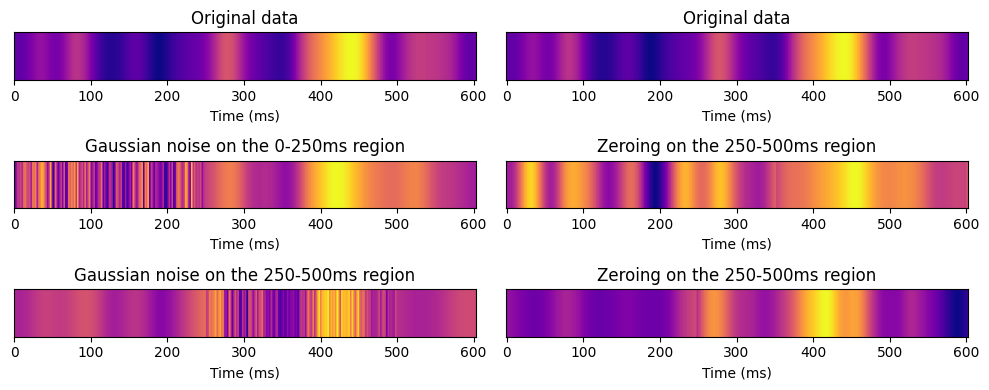
\includegraphics[width=7.7cm]{img/shap.png}
    \caption{A one-dimensional heatmap of the SHAP values of the variance had averaged over all channels on the original signal, a signal with noise in the 0-250ms region, and a signal with noise in the 250-500ms region. Lighter colors indicate a strong positive contribution, whereas darker colors indicate a strong negative contribution.}
    \label{fig:shap}
\end{figure}
